\newsavebox\neuralnet
\begin{lrbox}{\neuralnet}
  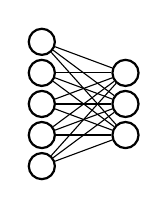
\begin{tikzpicture}
    \node[circle, thick, fill=white, draw] (x1) {};
    \node[circle, thick, fill=white, draw, below=0.1em of x1] (x2) {};
    \node[circle, thick, fill=white, draw, below=0.1em of x2] (x3) {};
    \node[circle, thick, fill=white, draw, above=0.1em of x1] (x4) {};
    \node[circle, thick, fill=white, draw, above=0.1em of x4] (x5) {};

    \node[circle, thick, fill=white, draw, right=2em of x1] (x11) {};
    \node[circle, thick, fill=white, draw, below=0.1em of x11] (x12) {};
    \node[circle, thick, fill=white, draw, above=0.1em of x11] (x13) {};

    \foreach \x in {1,...,5}
    \foreach \y in {1,...,3}
    \draw (x\x) -- (x1\y);
  \end{tikzpicture}
\end{lrbox}

\usetikzlibrary{calendar,fpu,matrix, positioning,arrows,arrows.meta,calc,decorations.pathreplacing,decorations.text,spy}
\tikzset{
  % style for inserting images as nodes
  img/.style={
      % text width=2cm, %% don't use this text height=2cm, %% don't use this
      inner sep=0pt,     % % use this
      outer sep=0pt,     % % and this
      rectangle,
      align=center} % only for debugging..
}

\tikzset{
  moon colour/.style={
      moon fill/.style={
          fill=#1
        },
      scale=0.5,
    },
  sky colour/.style={
      sky draw/.style={
          draw=#1
        },
      sky fill/.style={
          fill=#1
        }
    },
  southern hemisphere/.style={
      rotate=180
    }
}

\makeatletter
\pgfcalendardatetojulian{2010-01-15}{\c@pgf@counta} % 2010-01-15 07:11 UTC --
% http://aa.usno.navy.mil/cgi-bin/aa_moonphases.pl?year=2010&ZZZ=END
\def\synodicmonth{29.530588853}
\newcommand{\moon}[2][]{
  {
      \tikzset{external/export=false}
      \edef\checkfordate{\noexpand\in@{-}{#2}}
      \checkfordate
      \ifin@
        \pgfcalendardatetojulian{#2}{\c@pgf@countb}% %
        \pgfkeys{/pgf/fpu=true,/pgf/fpu/output format=fixed}% %
        \pgfmathsetmacro\dayssincenewmoon{\the\c@pgf@countb-\the\c@pgf@counta-(7/24+11/(24*60))}% %
        \pgfmathsetmacro\lunarage{mod(\dayssincenewmoon,\synodicmonth)}
        \pgfkeys{/pgf/fpu=false}% %
      \else
        \def\lunarage{#2}
      \fi
      \pgfmathsetmacro\leftside{ifthenelse(\lunarage<=\synodicmonth/2,cos(360*(\lunarage/\synodicmonth)),1)}% %
      \pgfmathsetmacro\rightside{ifthenelse(\lunarage<=\synodicmonth/2,-1,-cos(360*(\lunarage/\synodicmonth))}% %%
      \tikz [moon colour=white,sky colour=black,#1]{
        \draw [moon fill, sky draw] (0,0) circle [radius=1ex];
        \draw [sky draw, sky fill] (0,1ex)
        arc (90:-90:\rightside ex and 1ex)
        arc (-90:90:\leftside ex and 1ex)
        -- cycle;
      }% %%
    }
}
\newcommand{\newmoon}{\moon{0}}
\newcommand{\waxingcrescent}{\moon{\synodicmonth/8}}
\newcommand{\firstquartermoon}{\moon{2*\synodicmonth/8}}
\newcommand{\waxinggibbous}{\moon{3*\synodicmonth/8}}
\newcommand{\fullmoon}{\moon{4*\synodicmonth/8}}
\newcommand{\waninggibbous}{\moon{5*\synodicmonth/8}}
\newcommand{\thirdquartermoon}{\moon{6*\synodicmonth/8}}
\newcommand{\waningcrescent}{\moon{7*\synodicmonth/8}}
\newcommand{\shadowed}{\moon{8}}
\newcommand{\unshadowed}{\moon{16}}
\newcommand{\removespace}[1]{\!\!\!\!\!\!\!\!\!\!#1\!}